\scanpage{5}
\mspage{4}

veut que si $U$ \deleted{$(=C\unsure{)(|(}T)$} est à la fois modéré fini
et modéré cofini, donc si $S$ et $T$
sont \deleted{deux} parties modérées finies
\deleted{telles} disjointes telles que \deleted{\unsure{tout}} \inserted{a)} $S\cup T$
modéré i.e. \figure{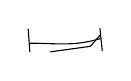
\begin{tikzpicture}[x=1cm,y=1cm]
\draw (0,.16)--(.02,-.13) (.91,.17)--(.94,-.12);
\draw (.01,-.02) to[out=0,in=197] (.92,.04);
\draw (.28,-.13)--(.79,-.06)--(.91,.08);
\end{tikzpicture}} $\unsure{s|S}\in S$ modéré p.r. à tt
$t\in T$, et b) Tout $u\in\mathcal L$ \unsure{modér.|modéré} p.r. à
$S$ est dans $T$\unsure{;|,}, \deleted{alors $S\cup T=\mathcal L$} et
à fortiori $S\cup T$ est partie \inserted{finie} modérée
maximale, donc $S\cup T=\mathcal L$, et
$\unsure{{}^{\cdot\cdot}S_0|S_0}=P_2(\mathcal L)$, enfin les relations
d'équivalence sont discrètes, et les
$\dot A$ sont vides. Pour le formuler,
on définit \unsure{la|a}

\deleted{Déf} \inserted{Ex 1} \uline{structure \inserted{de Réseau} discrète} sur $\mathcal L$

\[
 S_0=P_2(\mathcal L)\ \Longrightarrow\
 \left\{\begin{aligned}
 &\mathrm{Modf}(\unsure{\mathcal L|\mathcal L_0})=\deleted{\unsure{\mathrm{Mod}}}P_f(\mathcal L)\\
 &C_T=\mathcal L\setminus T\qquad\text{si }T\in P_f(\mathcal L)
 \end{aligned}\right.
\]

\[
\begin{aligned}
 &\deleted{C(T)=\unsure{\subset|\mathcal L}}\\
 &R_{\unsure{T|T\rceil|\Pi}}=\text{relation d'équivalence discrète}\\
 &\hspace{3em}\text{dans }\mathcal L\setminus T,\quad\text{donc les composantes}\\
 &\hspace{4em} \inserted{A}\ \text{sont réduites à un pt}\\
 &\deleted{\text{Pour Donc}}\\
 &\dot A=\varnothing
\end{aligned}
\]

\uline{Axiome}\quad Si $T$ est partie finie modérée
maximale, alors $T=\mathcal L$, $\mathcal L$ est \unsure{discrêt|discrèt|discret}.

% paper watermark, visible from the reverse
\rotatebox{90}{\textsc{\unsure{Strong Extra St}}}
